% Created 2022-12-03 Sat 22:24
% Intended LaTeX compiler: pdflatex
\documentclass[10pt, presentation, colorlinks]{beamer}
\usepackage[utf8]{inputenc}
\usepackage[T1]{fontenc}
\usepackage{graphicx}
\usepackage{longtable}
\usepackage{wrapfig}
\usepackage{rotating}
\usepackage[normalem]{ulem}
\usepackage{amsmath}
\usepackage{amssymb}
\usepackage{capt-of}
\usepackage{hyperref}
\usecolortheme{magpie}
\usepackage{minted}
\usemintedstyle{monokai}
\newminted{haskell}{}
\usetheme{default}
\author{Rebecca Skinner}
\date{2022-12-07}
\title{Building a Console Application in Haskell}
\AtBeginSection[]{\begin{frame}<beamer>\frametitle{}\center{\huge{\secname}}\end{frame}}
\hypersetup{
 pdfauthor={Rebecca Skinner},
 pdftitle={Building a Console Application in Haskell},
 pdfkeywords={},
 pdfsubject={},
 pdfcreator={Emacs 28.2 (Org mode 9.5.5)},
 pdflang={English}}
\begin{document}

\maketitle

\section{Prelude}
\label{sec:org77db2c3}

\begin{frame}[label={sec:org84d12ad}]{Hello, World}
\begin{itemize}
\item About Me: Rebecca Skinner
\begin{itemize}
\item Lead Software Engineer at Mercury
\item Author of Effective Haskell
\end{itemize}
\item @cercerilla on Twitter and Cohost
\item \url{https://rebeccaskinner.net}
\item \url{https://github.com/rebeccaskinner/}
\end{itemize}

\begin{center}

\includegraphics[height=0.3\textheight]{img/url.png}
\end{center}
\end{frame}

\begin{frame}[label={sec:orgafb926b}]{Effective Haskell}
\begin{columns}
\begin{column}[t]{0.45\columnwidth}
\begin{center}
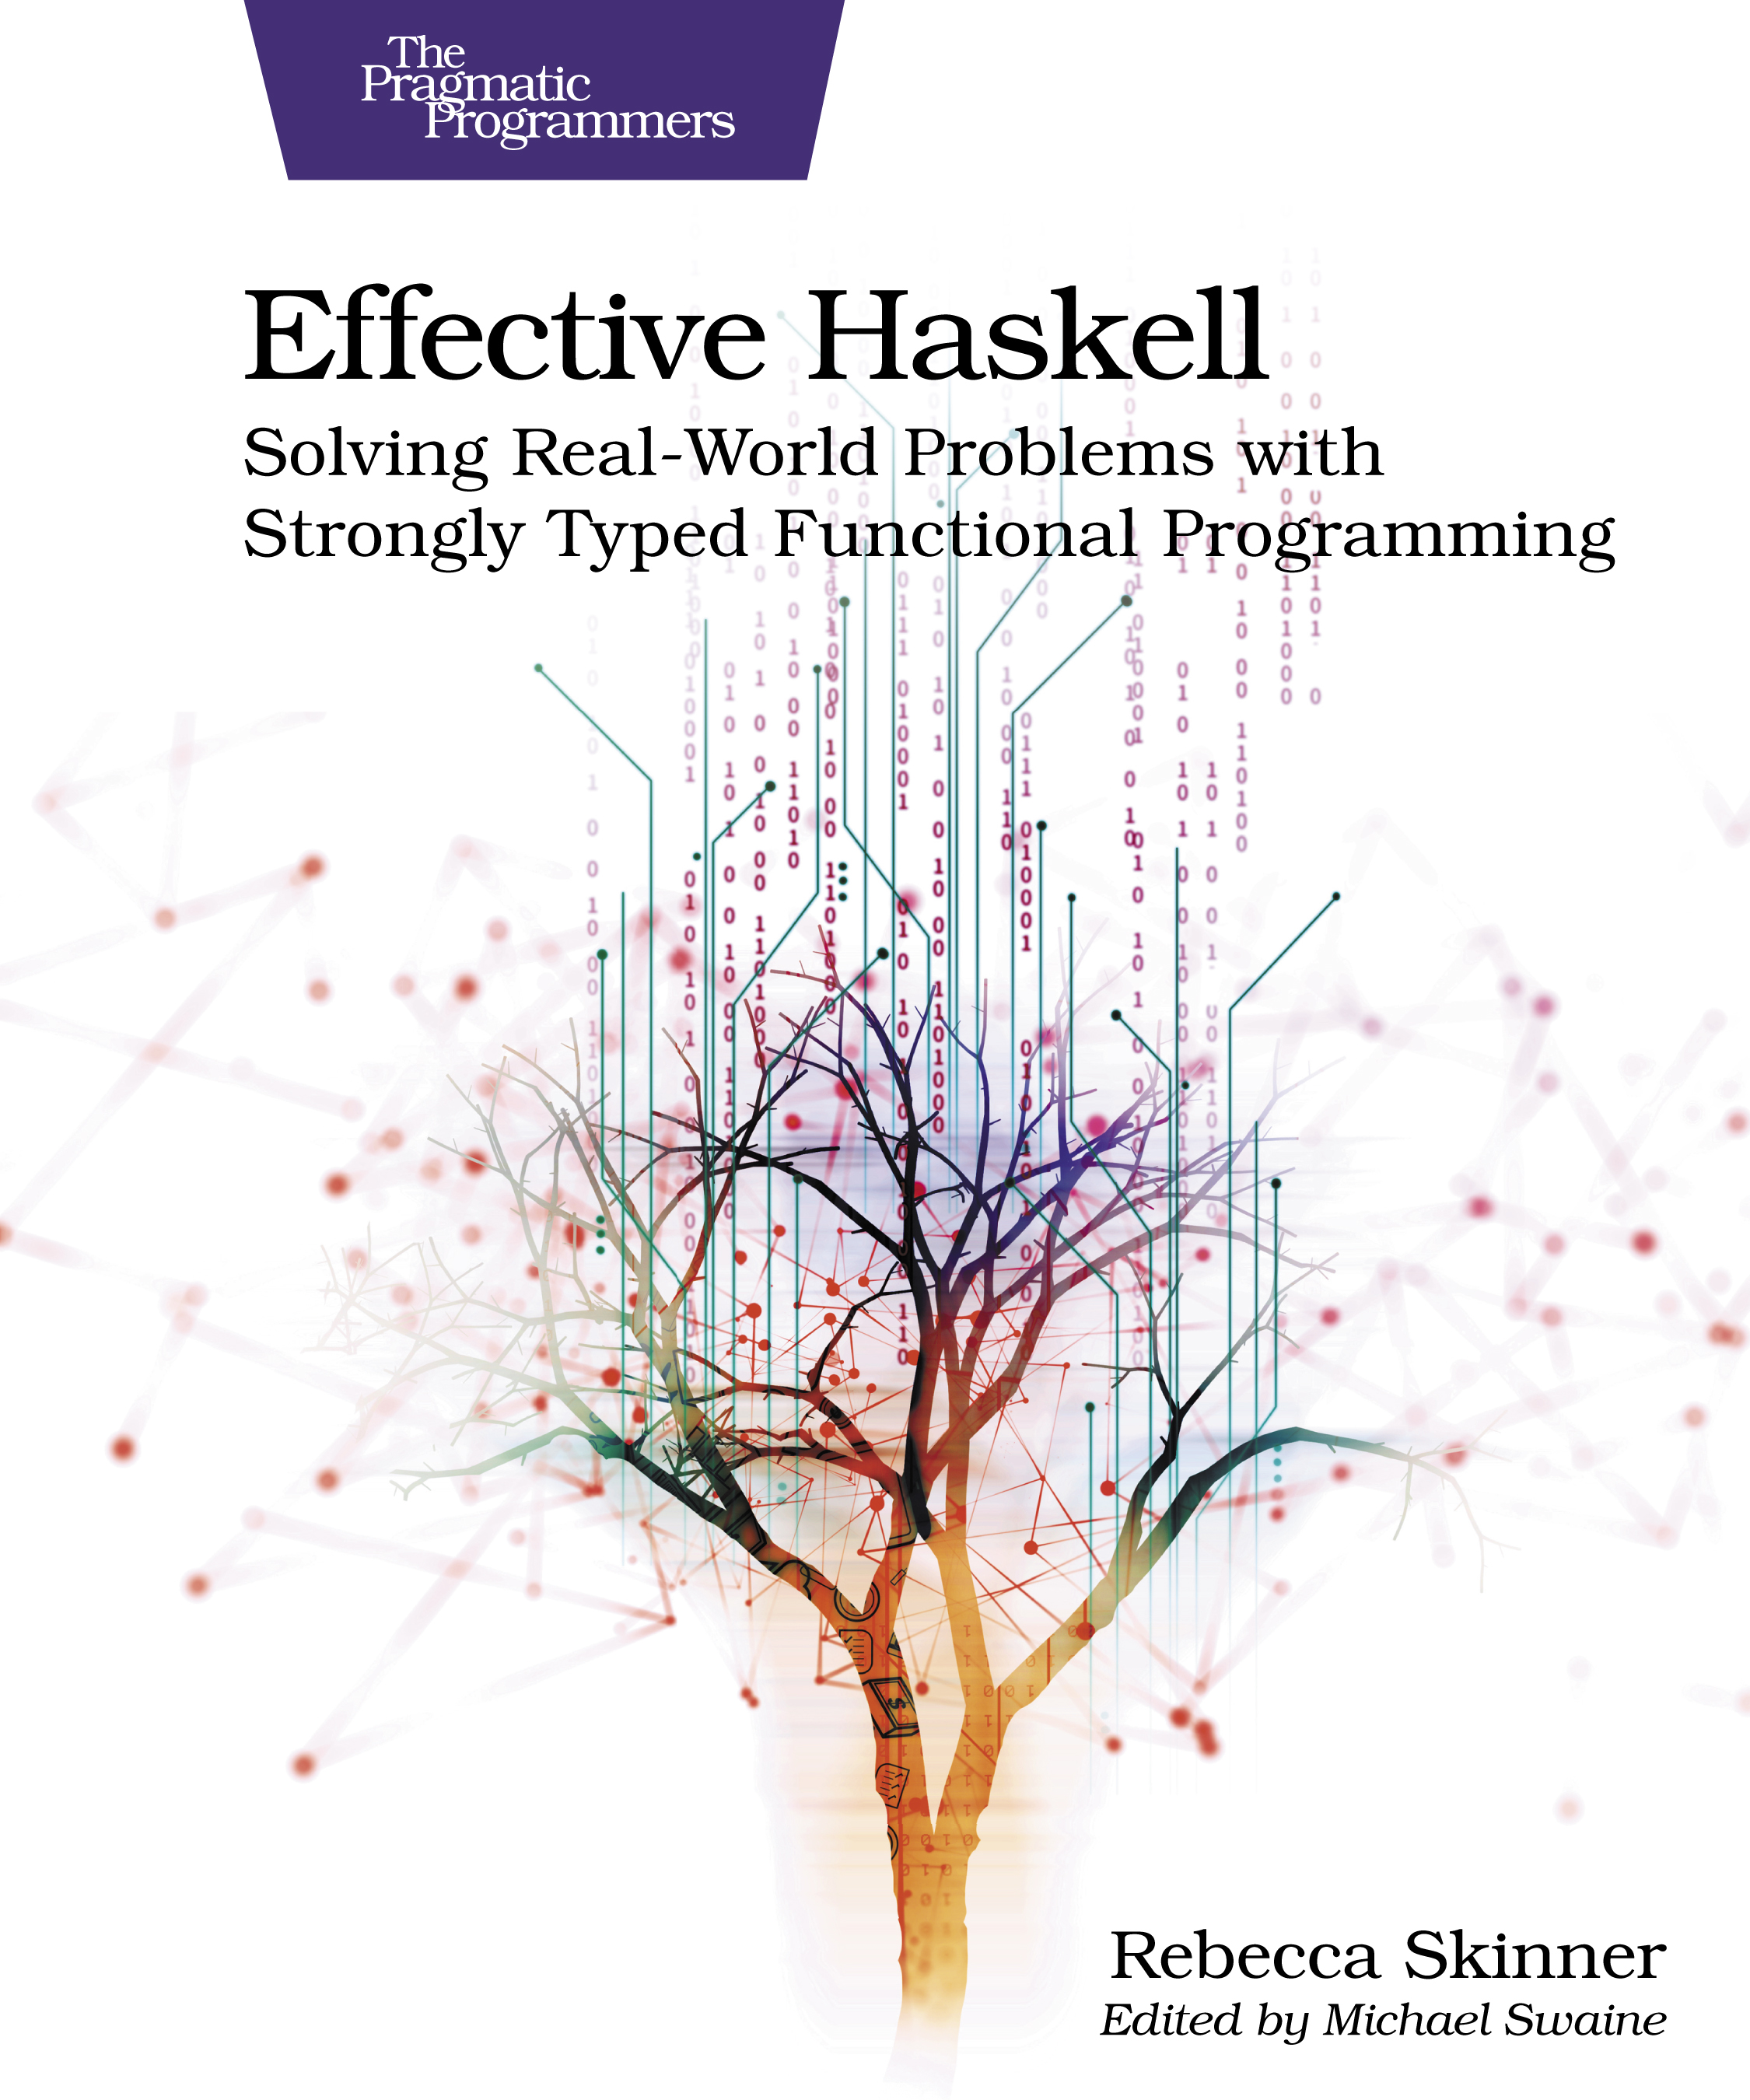
\includegraphics[height=0.7\textheight]{img/rshaskell.jpg}
\end{center}
\end{column}

\begin{column}[t]{0.45\columnwidth}
\begin{figure}[htbp]
\centering

\includegraphics[height=0.3\textheight]{img/effective-haskell-url.png}
{\tiny{https://tinyurl.com/2744kfu7\\ Now in Beta!}}
\end{figure}
\end{column}
\end{columns}
\end{frame}

\begin{frame}[label={sec:orgf8c53fa}]{About This Talk}
During this talk we're going to \uline{discover} how to build basic command
line tool in Haskell. As we go, you'll:

\bigskip

\begin{itemize}
\item Learn how Haskell programs use IO actions to deal with the real world
\item Find out how to do simple terminal and file IO
\item See examples of how to mix IO and pure functional code effectively
\item Follow along with implementing pure functional code to work with text
\end{itemize}

\bigskip

\alert{Most importantly}: You'll get an intuition for how to think about
building Haskell programs that can serve as a basis for future
learning.
\end{frame}

\begin{frame}[label={sec:org77d8925}]{HCat}
\begin{center}
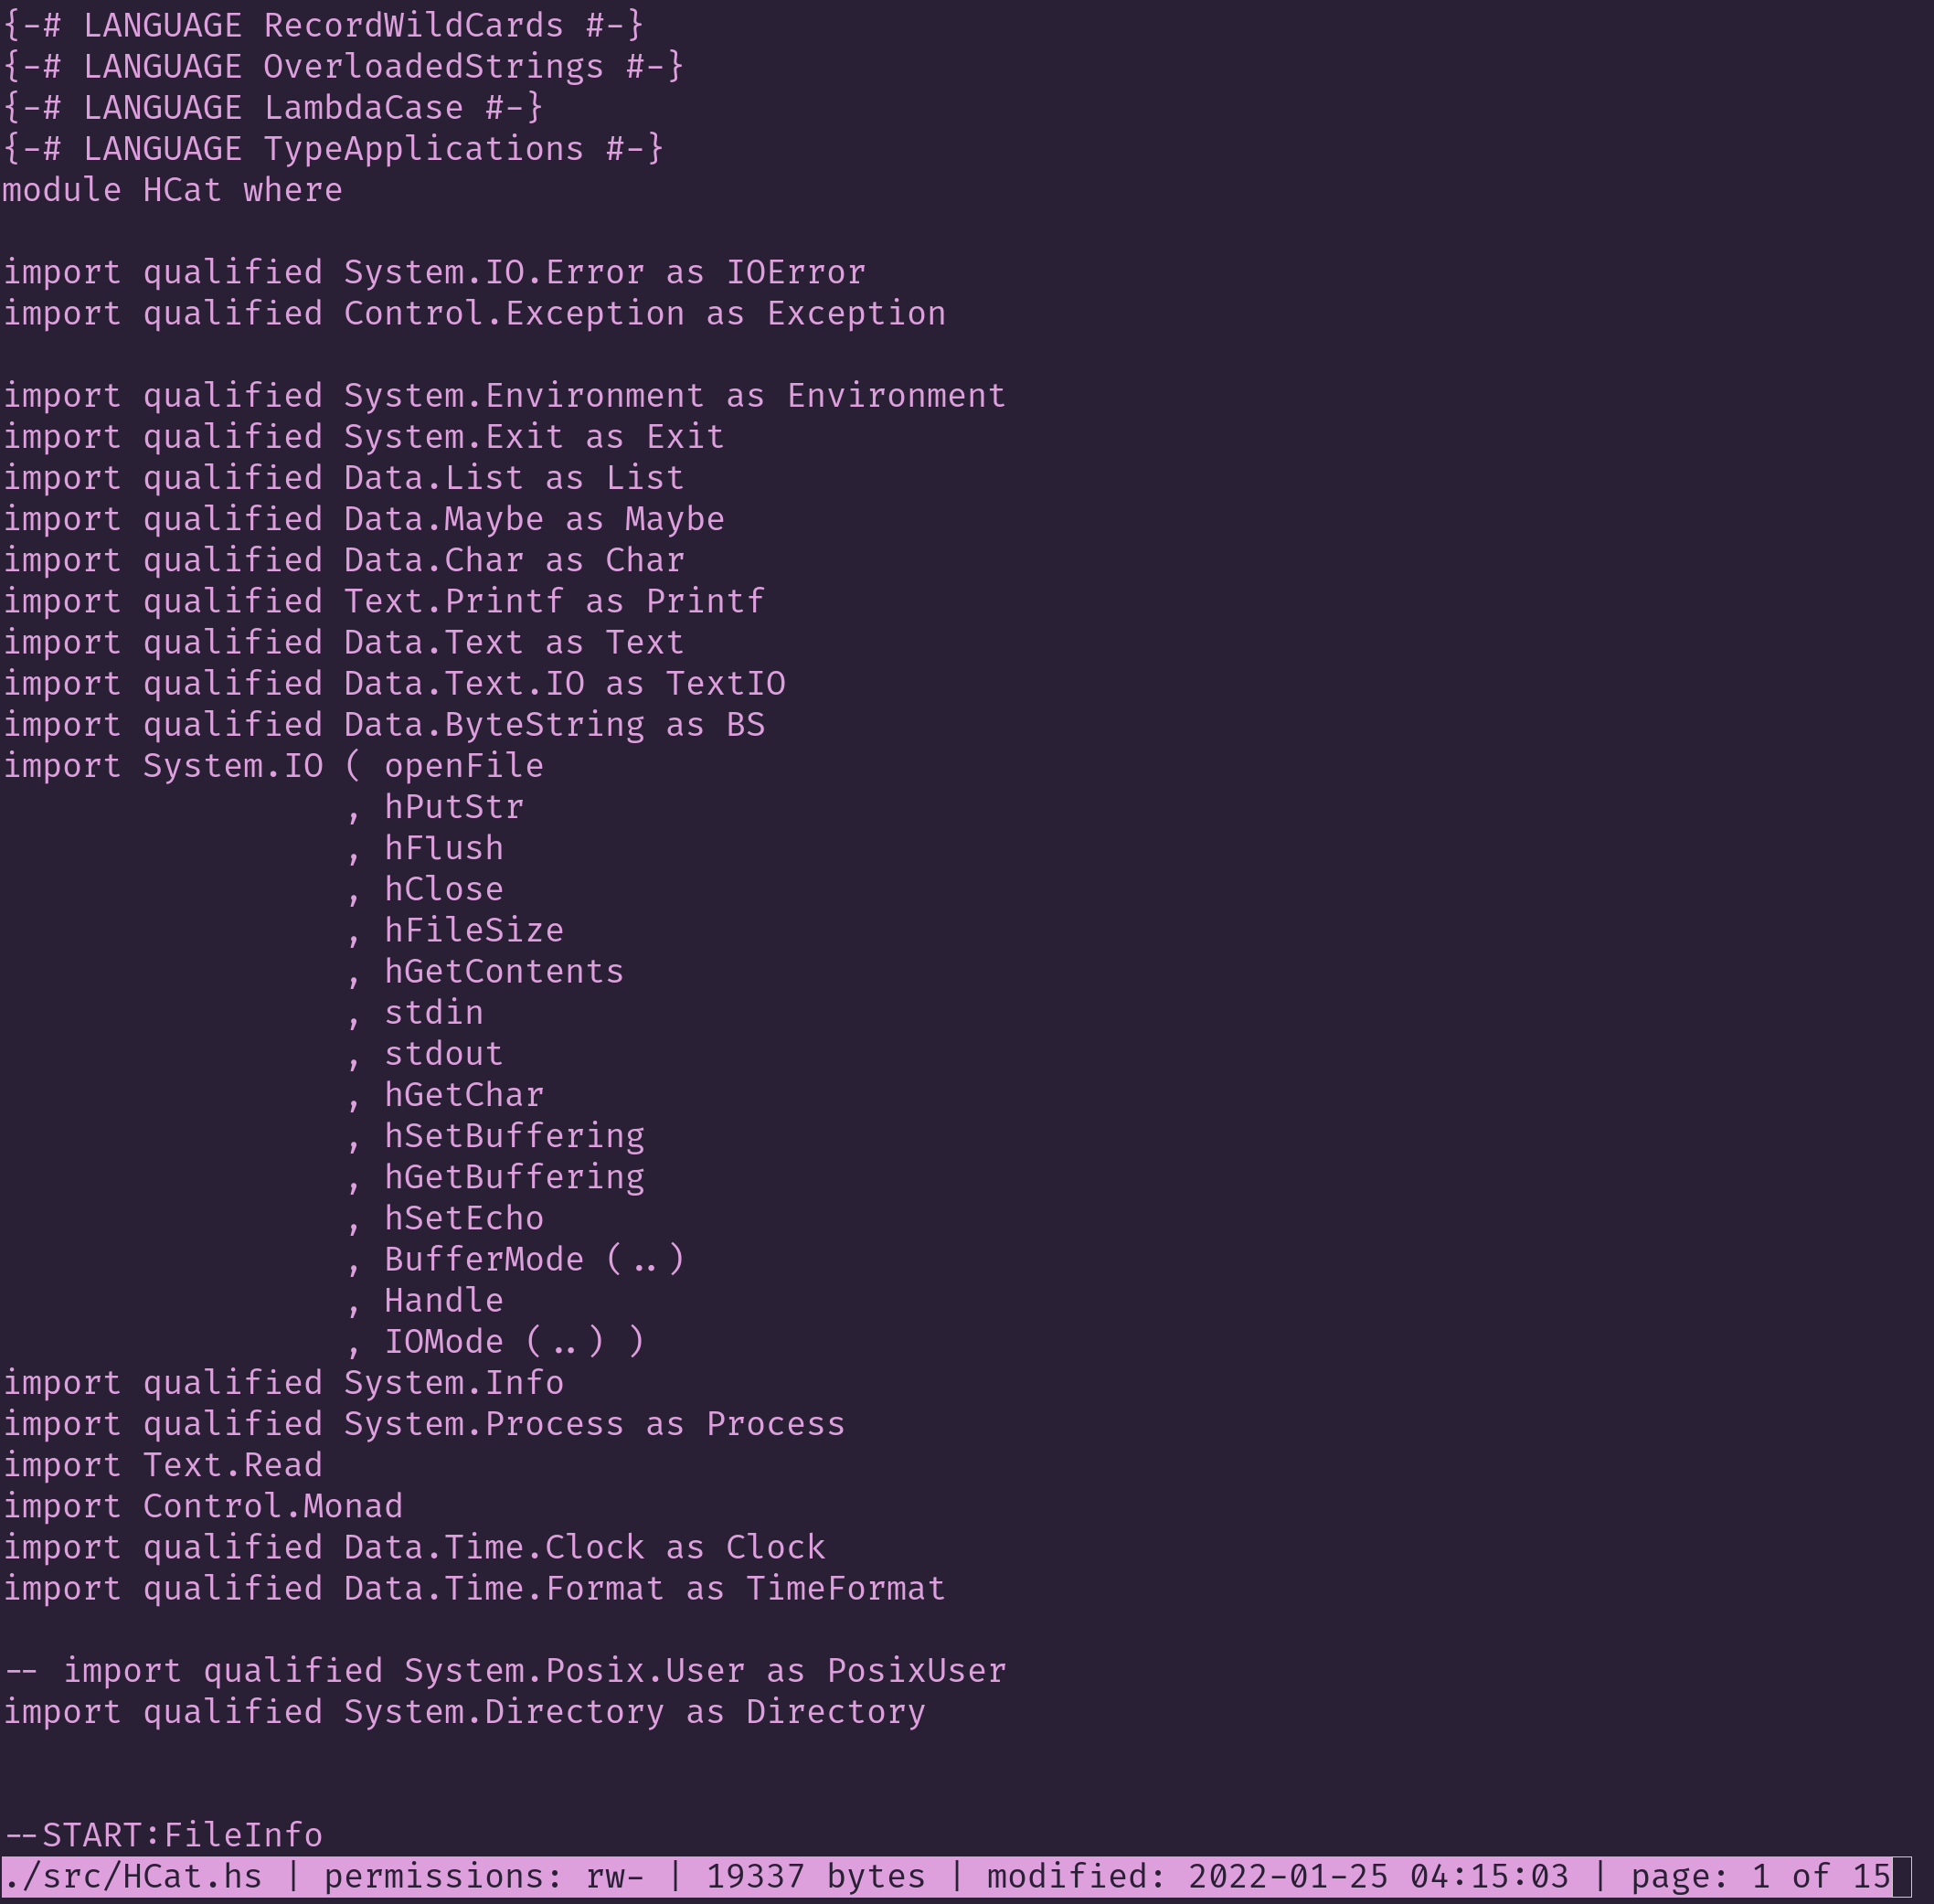
\includegraphics[height=0.7\textheight]{./img/hcat-screen.png}
\end{center}
\end{frame}

\section{Understanding IO}
\label{sec:orgc857986}

\begin{frame}[label={sec:org1b11d78}]{A True Color Photo of Side Effects}
\begin{center}

\includegraphics[height=0.6\textheight]{./img/io.jpg}
\end{center}
\center{A side effect in its natural environment.}
\end{frame}

\begin{frame}[label={sec:org9096779}]{The Trouble with IO}
Haskell is a \alert{pure functional} language, but most of the things we want our programs to do revolve around \alert{side effects}!

\bigskip

\pause
\begin{itemize}
\item Reading and writing files
\end{itemize}
\pause
\begin{itemize}
\item Printing text to the screen
\end{itemize}
\pause
\begin{itemize}
\item Handling user input
\end{itemize}
\end{frame}

\begin{frame}[label={sec:org6280334},fragile]{Can We Have a Little Bit of IO?}
 What if we cheat just a little?

\bigskip
\pause

\begin{minted}[frame=lines,fontsize=\scriptsize,linenos=false]{haskell}
writeReadFile =
  let
    _ = writeFile "example.txt" "Hello, Haskell"
    fileContents = readFile "example.txt"
  in print fileContents
\end{minted}

\bigskip

\pause
\begin{itemize}
\item Nothing will happen until we evaluate \texttt{writeReadFile}
\end{itemize}
\pause
\begin{itemize}
\item When we evaluate \texttt{writeReadFile} we'll get whatever random contents were in \texttt{example.txt}
\end{itemize}
\pause
\begin{itemize}
\item We won't ever write \alert{"Hello, Haskell"} to the file, because we're not using result of \texttt{writeFile}!
\end{itemize}
\end{frame}

\begin{frame}[label={sec:org1393aaa}]{Let's Dream of a Better Way}
\begin{center}

\includegraphics[height=0.6\textheight]{./img/dreaming.png}
\end{center}
\center{Let's dream up a better way}
\end{frame}

\begin{frame}[label={sec:org2258334}]{IO, the Lazy Way}
If we want to be lazy, we need to work for it by making sure every new
side effect \alert{must depend on} the previous one.

\begin{center}

\includegraphics[height=0.6\textheight]{./img/dominos.png}
\end{center}
\end{frame}

\begin{frame}[label={sec:org2f3f09a}]{Sometimes Things Are Easy}
In some cases, there is a natural dependency between side effects:

\bigskip
\pause
\begin{itemize}
\item Reading a file, then printing the contents
\end{itemize}

\bigskip
\pause
More often, there isn't an obvious dependency:

\bigskip
\pause
\begin{itemize}
\item Writing a log message before opening a file
\item Writing data to a file, then reading the contents
\item Printing a message to the screen then waiting on user input
\end{itemize}
\end{frame}

\begin{frame}[label={sec:orgaaa8417}]{A Pointer To The Real World}
We needed to \alert{sequence} our side effects correctly because there's an implicit data dependency we haven't considered: \alert{the state of the real world}.

\bigskip
\pause
\begin{center}

\includegraphics[height=0.4\textheight]{./img/pointing-to-the-real-world.png}
\end{center}
\center{\verb|data RealWorld}
\end{frame}

\begin{frame}[label={sec:orgf90afd3},fragile]{Welcome to the Real World}
 We can use a reference to the \texttt{RealWorld} to add a dependency between all of our calls:

\bigskip
\pause

\begin{minted}[frame=lines,fontsize=\scriptsize,linenos=false]{haskell}
writeReadFile world0 =
  let
    (world1, _) = writeFile world0 "example.txt" "Hello, Haskell"
    (world2, fileContents) = readFile world1 "example.txt"
  in print world2 fileContents
\end{minted}

\bigskip
\pause

But it sucks.
\end{frame}

\begin{frame}[label={sec:orgeda50f5}]{Typing IO Operations}
\begin{center}

\includegraphics[height=0.4\textheight]{./img/typewriter.JPG}
\end{center}
\center{Let's make a type!}
\end{frame}

\begin{frame}[label={sec:org0b1e226},fragile]{Typing IO Operations}
 \begin{minted}[frame=lines,fontsize=\scriptsize,linenos=false]{haskell}
data SideEffect a =
  SideEffect { runSideEffects :: RealWorld -> (RealWorld, a) }
\end{minted}
\end{frame}

\begin{frame}[label={sec:org5389a3c},fragile]{Side Effects Are Programs}
 Think of \texttt{SideEffect a} as a \alert{program} that returns a value of type
\texttt{a}.

\bigskip

\begin{description}
\item[{\texttt{SideEffect String}}] : A program that runs and outputs a \texttt{String}
\item[{\texttt{SideEffect Int}}] : A program that runs and outputs an \texttt{Int}
\end{description}

\bigskip

\texttt{SideEffect} programs are not pure functional programs. They rely on, and change, the \texttt{RealWorld}.
\end{frame}

\begin{frame}[label={sec:org6847513},fragile]{Side Effect Examples}
 Let's look at some examples of \texttt{SideEffect} programs. We'll imagine
some internal helper functions that will do the unsafe low level IO
operations:

\begin{minted}[frame=lines,fontsize=\scriptsize,linenos=false]{haskell}
readFile :: FilePath -> SideEffect String
readFile filename = SideEffect $ \realWorld ->
  let (realWorld', contents) = internalReadFile filename realWorld
  in (realWorld', contents)

writeFile :: FilePath -> String -> SideEffect ()
writeFile filename contents = SideEffect $ \realWorld ->
  let realWorld' = internalWriteFile filename contents realWorld
  in (realWorld', ())

print :: String -> SideEffect ()
print message = SideEffect $ \realWorld ->
  let realWorld' = internalPrint message realWorld
  in (realWorld', ())
\end{minted}
\end{frame}

\begin{frame}[label={sec:orgff5839f},fragile]{Combining Side Effects}
 A \texttt{SideEffect} program can do things that have side effects, like
reading from and writing to files, but that's pretty limiting. We can
do a lot more if we can have a \texttt{SideEffect} program that executes
other \texttt{SideEffect} programs and uses the results.

\begin{minted}[frame=lines,fontsize=\scriptsize,linenos=false]{haskell}
data SideEffect a =
  SideEffect { runSideEffects :: RealWorld -> (RealWorld, a) }

joinSideEffects :: SideEffect (SideEffect a) -> SideEffect a
joinSideEffects outerSideEffect = SideEffect $ \world ->
  let (world', innerSideEffect) = runSideEffects outerSideEffect world
  in runSideEffects innerSideEffect world'
\end{minted}
\end{frame}

\begin{frame}[label={sec:org76837b6},fragile]{First One, Then The Other}
 Most of the time, we want to write a \texttt{SideEffect} program that does
one side effect \alert{and then} does another one. It turns out that this is
just another way of saying that we have one \texttt{SideEffect} program that
calls the first effect, and uses it's value to call the second one:

\begin{minted}[frame=lines,fontsize=\scriptsize,linenos=false]{haskell}
data SideEffect a =
  SideEffect { runSideEffects :: RealWorld -> (RealWorld, a) }

sequenceSideEffects :: SideEffect a -> (a -> SideEffect b) -> SideEffect b
sequenceSideEffects sideEffect makeNextSideEffect =
  joinSideEffects $ SideEffect $ \world ->
    let (world', val) = runSideEffects sideEffect world
    in (world', makeNextSideEffect val)
\end{minted}
\end{frame}

\begin{frame}[label={sec:org84e10b6},fragile]{Write, Read, Print}
 Let's to to write our program again, using the things we've just built:

\begin{minted}[frame=lines,fontsize=\scriptsize,linenos=false]{haskell}
writeReadFile :: SideEffect ()
writeReadFile =
  writeFile "example.txt" "Hello, Haskell"
  `sequenceSideEffects` (\_ -> readFile "example.txt")
  `sequenceSideEffects` (\contents -> print contents)
\end{minted}

\bigskip

How does this version compare?

\bigskip

\pause
\begin{itemize}
\item Every side effect depends on its predecessor, so they all happen in the right order
\end{itemize}
\pause
\begin{itemize}
\item Our code is focused on the work it needs to do, without having to explicitly pass around references to the real world
\end{itemize}
\pause
\begin{itemize}
\item Our code program is still a \alert{pure functional program}. Instead of doing side effects directly, we \alert{generate a program} that would have side effects if it were run. The programs themselves are still pure values.
\end{itemize}
\end{frame}

\begin{frame}[label={sec:org870319b}]{That's Not All}
\center{Before we get back to HCat}

\pause
\begin{center}
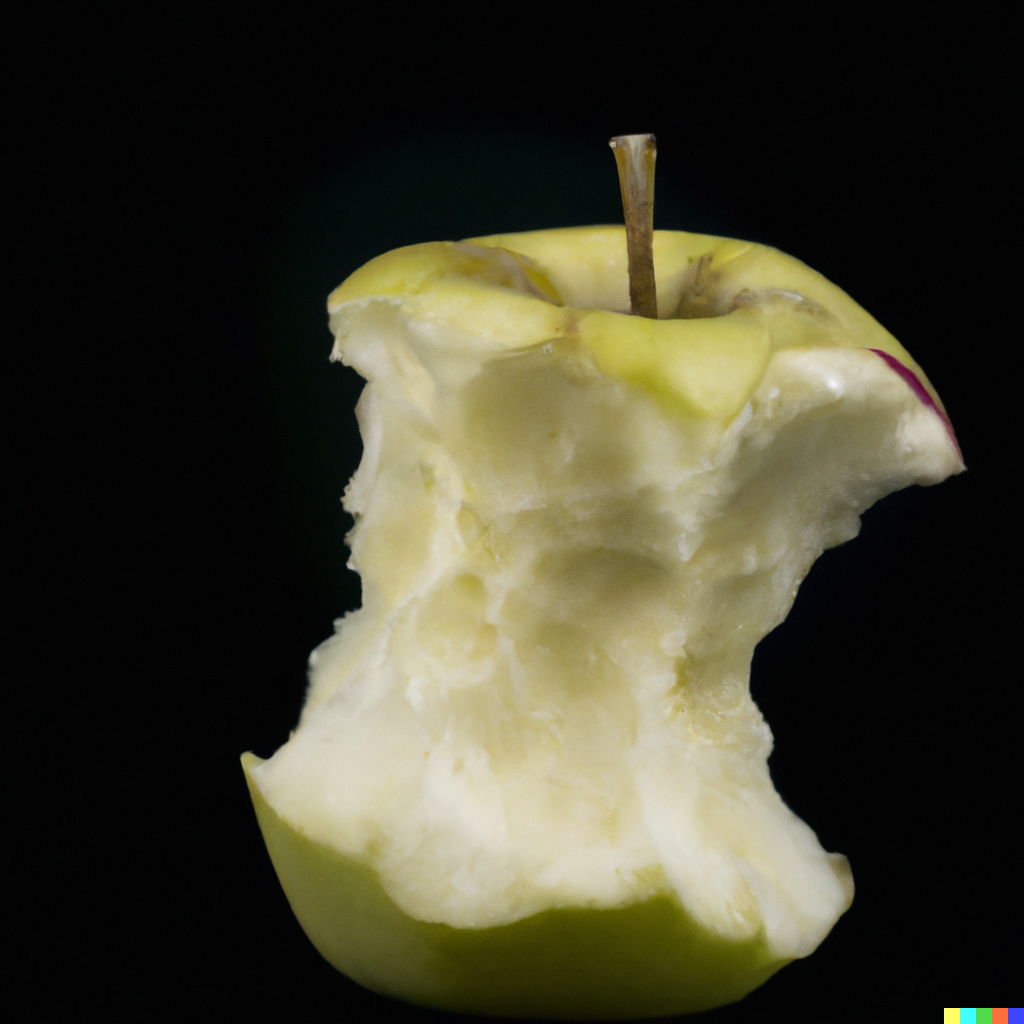
\includegraphics[height=0.5\textheight]{./img/apple.png}
\end{center}

\center{One more thing}
\end{frame}

\begin{frame}[label={sec:org0f3bde2}]{That's No Side Effect}
\begin{center}
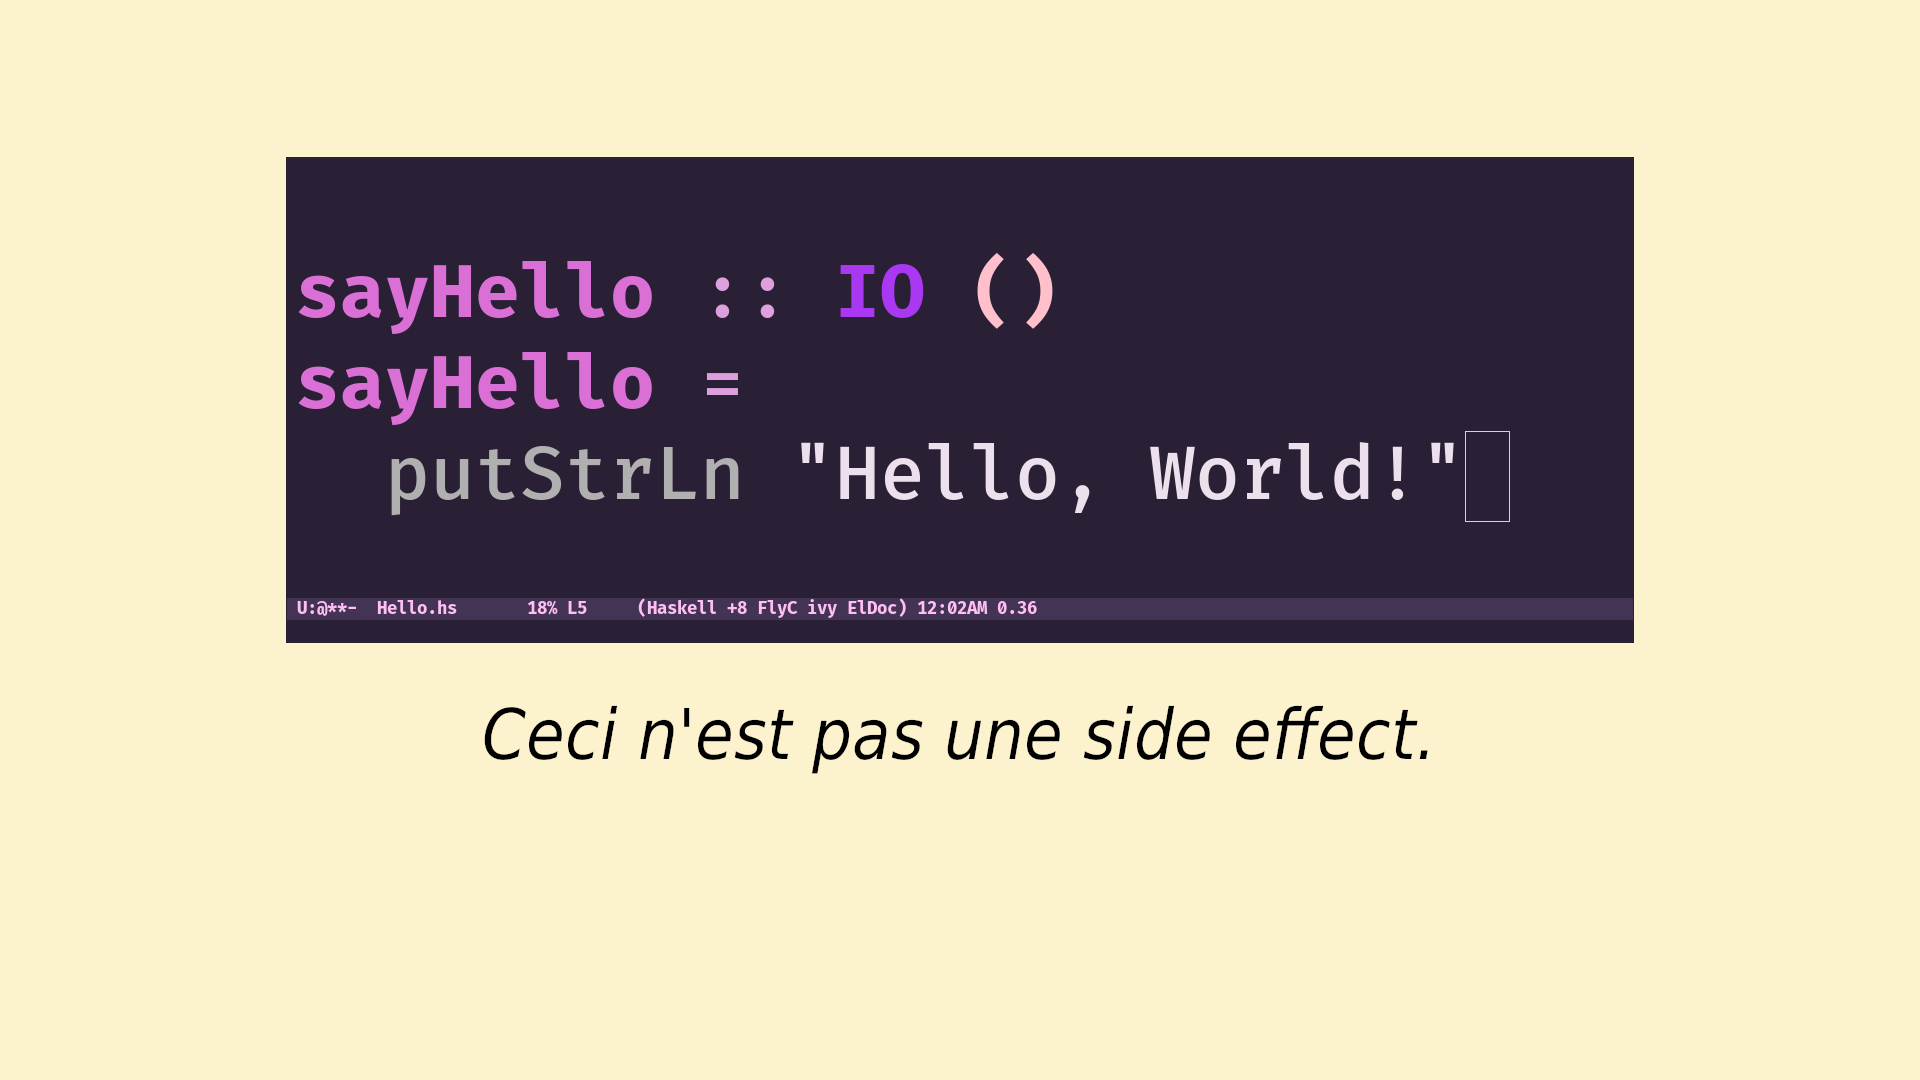
\includegraphics[height=0.6\textheight]{./img/no-side-effects.png}
\end{center}
\end{frame}

\begin{frame}[label={sec:org0be5fe8},fragile]{That's No Side Effect}
 It turns out our imaginary \texttt{SideEffect} type isn't entirely imaginary.

\pause
\begin{itemize}
\item Instead of \alert{\texttt{SideEffect a}} we say \alert{\texttt{IO a}}
\end{itemize}
\pause
\begin{itemize}
\item Instead of \alert{\texttt{sequenceSideEffects}} we say \alert{\texttt{>>=}}
\end{itemize}
\pause
\begin{itemize}
\item Instead of \alert{\texttt{SideEffect} program} we say \alert{\texttt{IO} action}
\end{itemize}
\pause

\begin{minted}[frame=lines,fontsize=\scriptsize,linenos=false]{haskell}
writeReadFile :: IO ()
writeReadFile =
  writeFile "example.txt" "Hello, Haskell"
  >>= (\_ -> readFile "example.txt")
  >>= print
\end{minted}
\end{frame}

\begin{frame}[label={sec:org68e771e},fragile]{To \alert{\texttt{do}} List}
 Writing a long chain of calls to \alert{\texttt{>>=}} gets tiresome. Instead we can
use \alert{\texttt{do} notation}:

\begin{minted}[frame=lines,fontsize=\scriptsize,linenos=false]{haskell}
writeReadFile :: IO ()
writeReadFile = do
  writeFile "example.txt" "Hello, Haskell"
  contents <- readFile "example.txt"
  print contents
\end{minted}

\pause
\begin{itemize}
\item Each line in a \alert{\texttt{do}} block corresponds to \alert{\texttt{>>=}}
\end{itemize}
\pause
\begin{itemize}
\item The \alert{\texttt{<-}} arrow names the output of an IO action
\end{itemize}
\pause
\begin{itemize}
\item When we run a Haskell program, the initial state of the real world
is used to run an IO action named \alert{\texttt{main}}.
\end{itemize}
\end{frame}

\section{HCat}
\label{sec:orgfc16f64}

\begin{frame}[label={sec:org501ed10}]{Return of the HCat}
\begin{center}

\includegraphics[height=0.6\textheight]{./img/return-of-the-hcat.png}
\end{center}
\end{frame}

\begin{frame}[label={sec:org7390aa9},fragile]{Back To The Code}
 Now that we understand how to write code that has side effects and
interacts with the real world, let's put it to practice with an \alert{MVP}:

\bigskip
\pause

\begin{minted}[frame=lines,fontsize=\scriptsize,linenos=false]{haskell}
module Main where

main :: IO ()
main = readFile "example.txt" >>= putStrLn
\end{minted}
\end{frame}

\begin{frame}[label={sec:org5332945}]{The M-est of MVPs}
\alert{Success!} we can read a file and print it out to the screen!

\bigskip
\pause
\ldots{}but only a single hard-coded file

\bigskip
\pause
\ldots{}and it's not actually paginated

\bigskip
\pause
\ldots{}or formatted for our terminal window

\bigskip
\pause
Let's take one problem at a time
\end{frame}

\begin{frame}[label={sec:orgc4d88dc}]{Getting Into Arguments}
\begin{center}

\includegraphics[height=0.6\textheight]{./img/arguments.png}
\end{center}
\center{we need to deal with arguments}
\end{frame}

\begin{frame}[label={sec:org2510d4e},fragile]{Getting Into Arguments}
 We can use \alert{\texttt{getArgs}} to get command line arguments, but we'll need to
deal with user errors.

\bigskip
\pause

\begin{minted}[frame=lines,fontsize=\scriptsize,linenos=false]{haskell}
module HCatArgs where
import System.Environment

targetFileName :: IO FilePath
targetFileName = do
  args <- getArgs
  case args of
    [filename] ->
      pure filename
    _otherwise ->
      ioError $ userError "please provide a single filename"

main :: IO ()
main = do
  contents <- readFile =<< targetFileName
  putStrLn contents
\end{minted}
\end{frame}

\begin{frame}[label={sec:org1e3080a},fragile]{Error Handling in IO Actions}
 Dealing with errors in IO actions can be complicated because there are a lot of options:

\bigskip
\pause

\begin{itemize}
\item Plain IO Errors
\item Using \texttt{Either} or \texttt{Maybe} values for failure
\item Custom exceptions
\item Monad Transformers
\end{itemize}

\bigskip
\pause

\alert{Opinion}: Getting too fancy too early will cause more problems than it solves. Start with the simplest thing that can possibly work.
\end{frame}

\begin{frame}[label={sec:org4aa4dfe}]{What About Libraries?}
Why parse arguments directly instead of using a library?

\bigskip
\pause

\begin{itemize}
\item Handling arguments yourself is good practice while learning
\item Some good libraries use language features you probably haven't learned yet
\end{itemize}
\end{frame}

\begin{frame}[label={sec:org2b6da65},fragile]{Terminal Size}
 The size of our terminal will determine our page count. We can get the terminal size with the \alert{\texttt{tput}} program on *nix systems.

\pause

\begin{minted}[frame=lines,fontsize=\scriptsize,linenos=false]{haskell}
module HCat where
import System.Process
data TerminalDimension = TerminalLines | TerminalCols
data ScreenDimensions =
  ScreenDimensions {screenRows :: Int, screenColumns :: Int}

getTerminalSize :: IO ScreenDimensions
getTerminalSize = do
  termLines <- tput TerminalLines
  termCols <- tput TerminalCols
  pure ScreenDimensions
    { screenRows = termLines
    , screenColumns = termCols }

tput :: TerminalDimension -> IO Int
tput dimension = do
  outputData <- readProcess "tput" [cmd] ""
  pure . read . head . lines $ outputData
  where
    cmd = case dimension of
      TerminalLines -> "lines"
      TerminalCols -> "cols"
\end{minted}
\end{frame}

\begin{frame}[label={sec:orgfb181e1},fragile]{Word Wrapping}
 Given the size of our terminal, we can wrap the text to fit.

\pause
\bigskip

\begin{minted}[frame=lines,fontsize=\scriptsize,linenos=false]{haskell}
wordWrap :: Int -> String -> [String]
wordWrap lineLength lineText =
  case splitAt lineLength lineText of
    (fullLine, "") -> [fullLine]
    (hardwrappedLine, rest) ->
      let (nextLine, remainder) = softWrap hardwrappedLine
       in nextLine : wordWrap lineLength (remainder <> rest)
  where
    softWrap hardWrapped =
      let (rest, wrappedText) = break isSpace $ reverse hardWrapped
       in (reverse wrappedText, reverse rest)

main :: IO ()
main = do
  contents <- readFile =<< targetFileName
  termSize <- getTerminalSize
  let wrapped = wordWrap (screenColumns termSize) contents
  putStrLn $ unlines wrapped
\end{minted}
\end{frame}

\section{Stepping Back}
\label{sec:orgddb9608}

\begin{frame}[label={sec:orga119089}]{Stepping Back}
\begin{center}
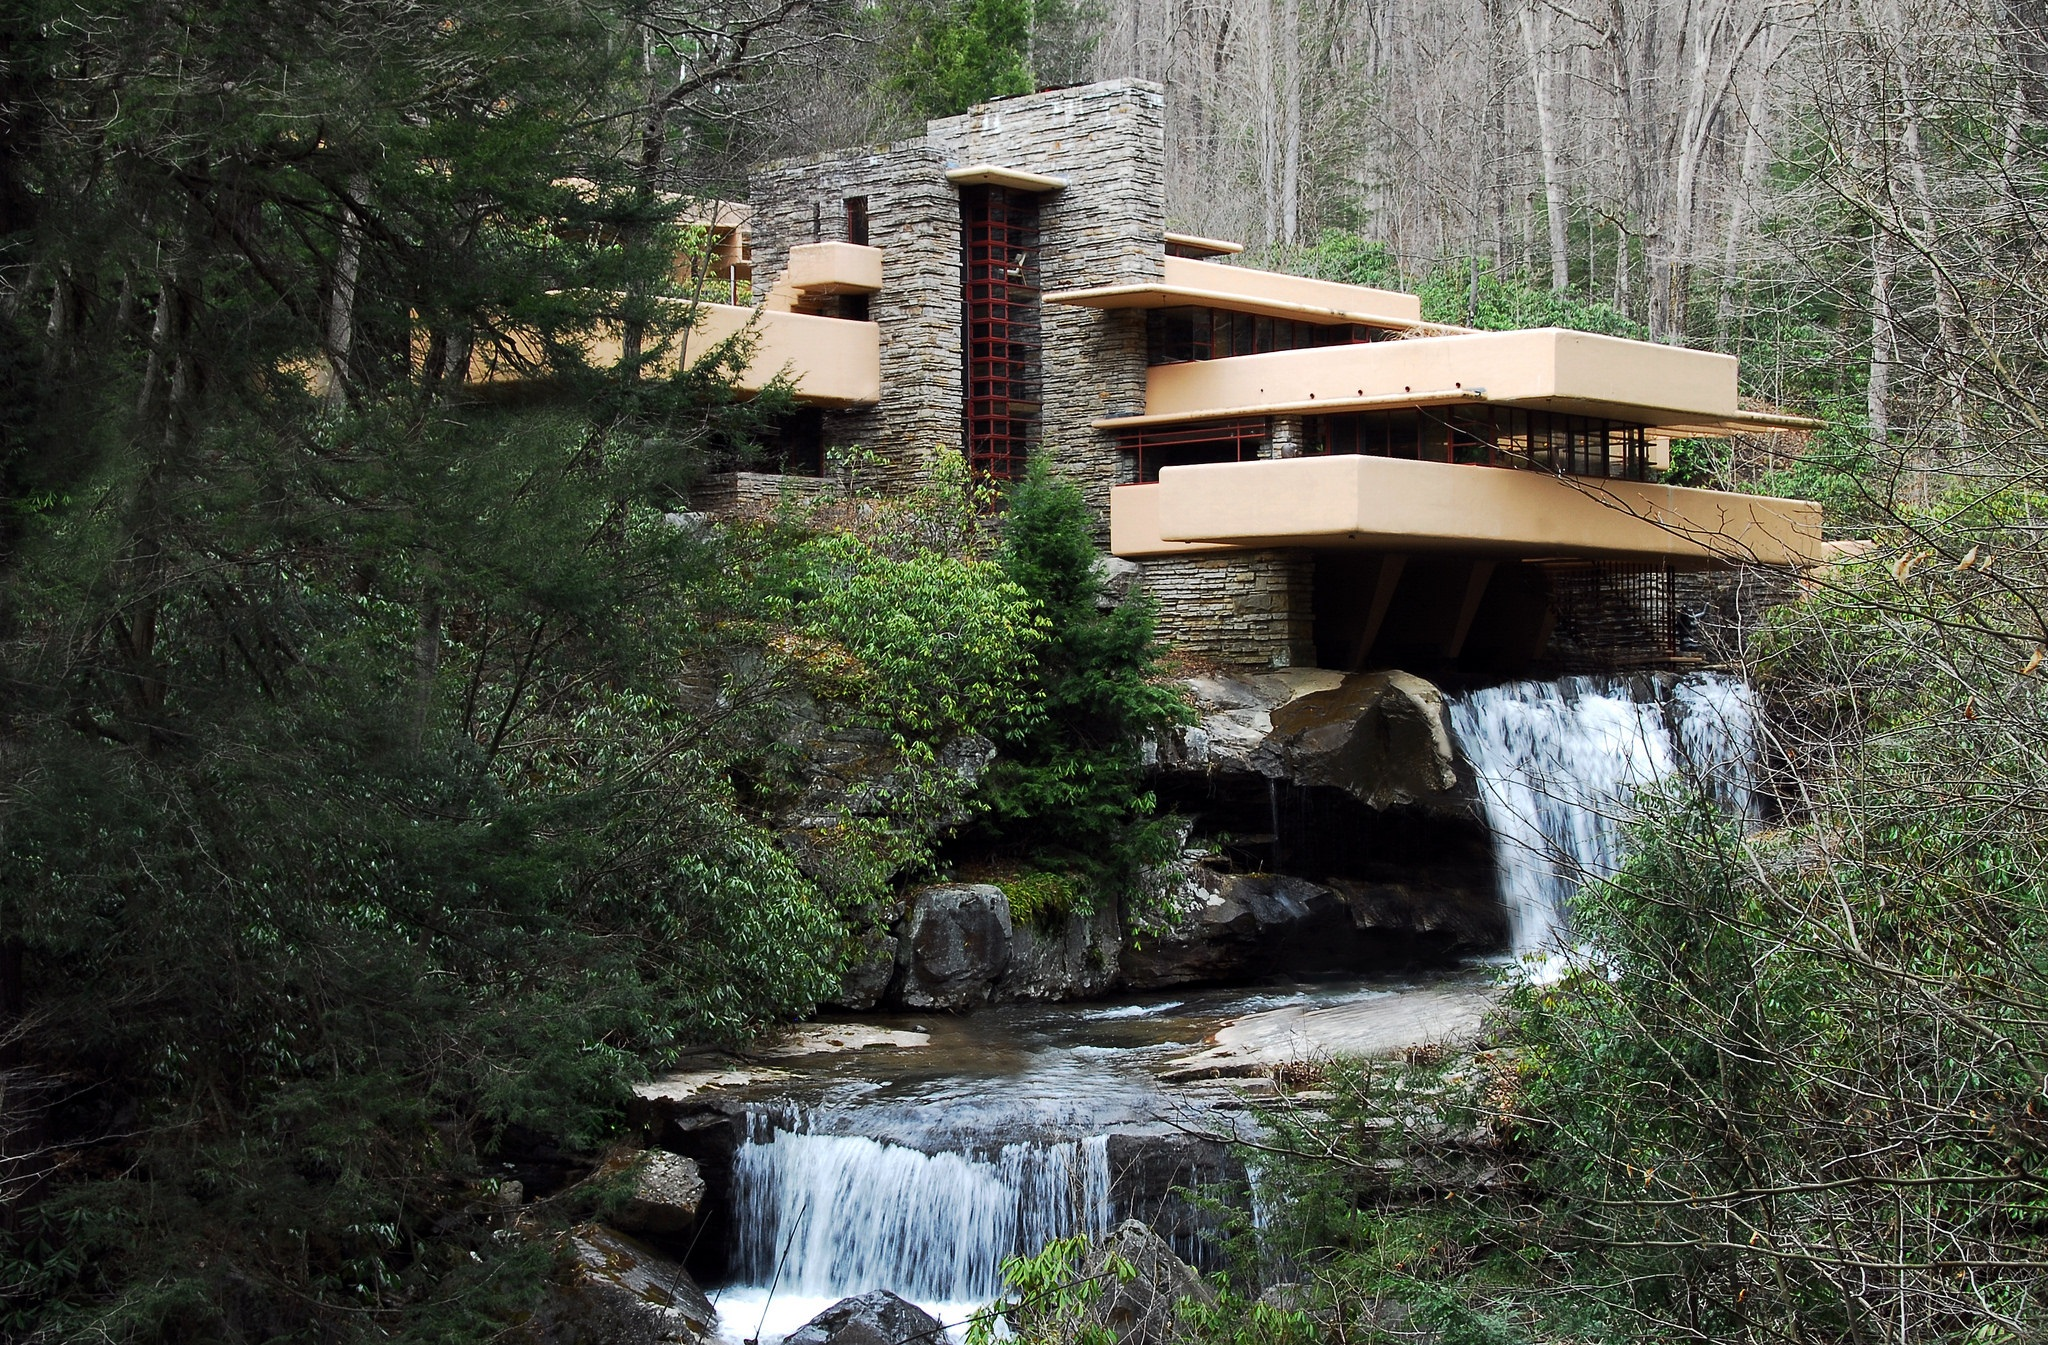
\includegraphics[height=0.6\textheight]{./img/architecture.jpg}
\end{center}
\center{Let's talk about Architecture}
\end{frame}

\begin{frame}[label={sec:org69fa52c},fragile]{A Tale of Two Word Wraps}
 In our earlier example, we built an IO action to fetch the terminal size, and passed the width into a \alert{pure function} that handled word wrapping. Let's consider the alternative:

\pause

\begin{minted}[frame=lines,fontsize=\scriptsize,linenos=false]{haskell}
wordWrap :: String -> IO [String]
wordWrap lineText = do
  lineLength <- tput TerminalCols
  case splitAt lineLength lineText of
    (fullLine, "") ->
      pure [fullLine]
    (hardwrappedLine, rest) -> do
      let (nextLine, remainder) = softWrap hardwrappedLine
      wrappedRemainder <- wordWrap (remainder <> rest)
      pure (nextLine : wrappedRemainder)
  where
    softWrap hardWrapped =
      let (rest, wrappedText) = break isSpace $ reverse hardWrapped
       in (reverse wrappedText, reverse rest)
\end{minted}

\pause
This might look \alert{easier} at first. It hides details from the caller
behind a smaller interface, but now it can't be used from any pure
functions.
\end{frame}

\begin{frame}[label={sec:orgceb9b28}]{The Lesson}
As much as possible, have IO actions gather data then pass it into
pure functions for computation.
\end{frame}

\begin{frame}[label={sec:org8cade50}]{Procedural Shell, Functional Core}
\begin{center}
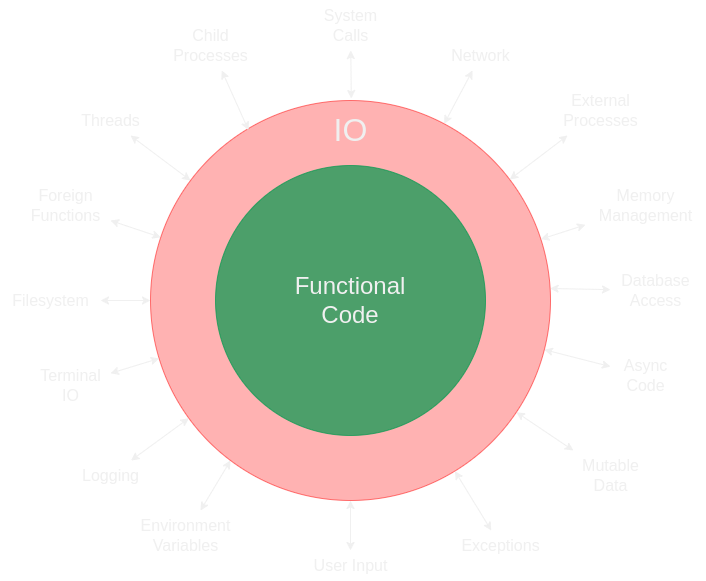
\includegraphics[height=0.6\textheight]{./img/functional-core.png}
\end{center}
\center{\tiny{The "procedural shell, functional core" model is an over-simplification of a good guideline}}
\end{frame}

\begin{frame}[label={sec:org41f20a5}]{IO Actions are Like Layers}
\begin{center}
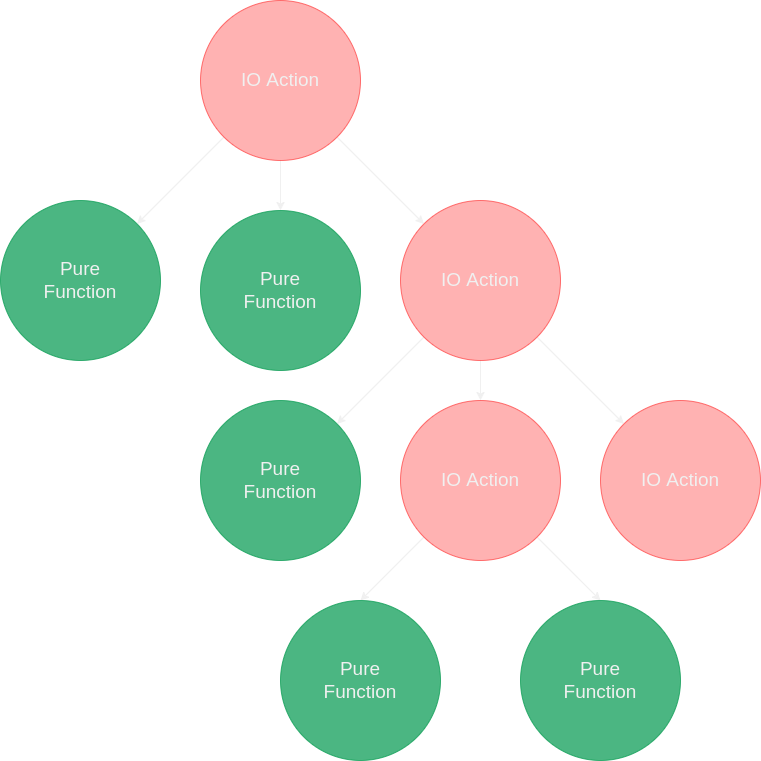
\includegraphics[height=0.6\textheight]{img/tree.png}
\end{center}
\center{\tiny{IO Actions and pure functions more closely resemble a tree}}
\end{frame}

\section{Back to HCat}
\label{sec:org7ea4465}

\begin{frame}[label={sec:org0cbfa71}]{Back to HCat}
\begin{center}

\includegraphics[height=0.6\textheight]{img/regularly-scheduled-hcat.png}
\end{center}
\center{\tiny{Back to our regularly scheduled HCat Presentation}}
\end{frame}

\begin{frame}[label={sec:org4ad1fc9},fragile]{Pagination}
 Our pager has one big problem right now: It doesn't \alert{paginate}.

\bigskip
\pause

\begin{minted}[frame=lines,fontsize=\scriptsize,linenos=false]{haskell}
paginate :: ScreenDimensions -> String -> [String]
paginate dimensions text = pages
  where
    rows = screenRows dimensions
    cols = screenColumns dimensions
    wrappedLines = concatMap (wordWrap cols) (lines text)
    pages = map (unlines . padTo rows) $ groupsOf rows wrappedLines
    padTo lineCount rowsToPad =
      take lineCount $ rowsToPad <> repeat ""
    groupsOf n elems
      | null elems = []
      | otherwise =
        let (hd, tl) = splitAt n elems
        in hd : groupsOf n tl
\end{minted}
\end{frame}

\begin{frame}[label={sec:orgd0a5b87}]{The Event Loop}
If we want to show our user a page at a time, we need to do a few things:

\bigskip
\pause

\begin{itemize}
\item Get some user input
\end{itemize}
\pause
\begin{itemize}
\item Loop over each page, displaying them
\end{itemize}
\pause
\begin{itemize}
\item Exit cleanly if the user wants to quit
\end{itemize}
\end{frame}

\begin{frame}[label={sec:org47b54fb},fragile]{Getting User Input}
 \begin{minted}[frame=lines,fontsize=\scriptsize,linenos=false]{haskell}
data ContinueCancel
  = Continue
  | Cancel
  deriving stock (Eq, Show)

getContinue :: IO ContinueCancel
getContinue = do
  hSetBuffering stdin NoBuffering
  hSetEcho stdin False
  input <- getChar
  case input of
    ' ' -> return Continue
    'q' -> return Cancel
    _ -> getContinue
\end{minted}
\end{frame}

\begin{frame}[label={sec:orgc9cbf36},fragile]{Taking User Input for a Loop}
 IO actions feel like a procedural language. Sometimes it's tempting to
fall back on familiar patterns. We even have access to things like
\alert{for} loops that make it easier to think this way.

\bigskip
\pause

\begin{minted}[frame=lines,fontsize=\scriptsize,linenos=false]{haskell}
showPages :: [String] -> IO ()
showPages allPages =
  for_ allPages $ \page -> do
    putStr "\^[[1J\^[[1;1H"
    putStr page
    cont <- getContinue
    -- ...
\end{minted}

\bigskip
\pause

Unfortunately, this can make things more difficult instead of easier.
\end{frame}

\begin{frame}[label={sec:org2adec6f},fragile]{Recursive IO Actions}
 You can use recursion in IO actions just like you would for pure
functions.

\bigskip
\pause

\begin{minted}[frame=lines,fontsize=\scriptsize,linenos=false]{haskell}
showPages :: [String] -> IO ()
showPages [] = pure ()
showPages (page:pages) = do
  putStr "\^[[1J\^[[1;1H"
  putStr page
  cont <- if null pages
          then pure Cancel
          else getContinue
  when (Continue == cont) $
    showPages pages
\end{minted}

\bigskip
\pause

This is a good starting spot for implementing the effectful logic in
your programs.
\end{frame}

\begin{frame}[label={sec:org18731fc}]{Continued Action}
As your programs grow, it's a good idea to think about making your IO
actions compose. This can make your code a bit more verbose at first,
but it buys you flexibility later.
\end{frame}

\begin{frame}[label={sec:org12a6705},fragile]{Continued Action}
 \alert{\texttt{onContinue}} lets us to do any IO action when the user continues:
\pause

\begin{minted}[frame=lines,fontsize=\scriptsize,linenos=false]{haskell}
onContinue :: IO () -> IO ()
onContinue ioAction = do
  cont <- getContinue
  case cont of
    Cancel -> pure ()
    Continue -> ioAction
\end{minted}
\pause

\alert{\texttt{forPages}} separates looping application logic with a \alert{continuation}:

\pause
\begin{minted}[frame=lines,fontsize=\scriptsize,linenos=false]{haskell}
forPages :: (String -> IO ()) -> [String]  -> IO ()
forPages ioAction pages  =
  case pages of
    [] -> pure ()
    (page:rest) -> do
      ioAction page
      onContinue (forPages ioAction rest)
\end{minted}
\pause

\alert{\texttt{showPages}} composes benefits from the work we've done

\pause
\begin{minted}[frame=lines,fontsize=\scriptsize,linenos=false]{haskell}
showPages :: [String] -> IO ()
showPages = forPages $ \page -> do
  putStr "\^[[1J\^[[1;1H"
  putStr page
\end{minted}
\end{frame}

\begin{frame}[label={sec:org5b66db6},fragile]{Putting It All Together}
 \begin{minted}[frame=lines,fontsize=\scriptsize,linenos=false]{haskell}
main :: IO ()
main = do
  contents <- readFile =<< targetFileName
  termSize <- getTerminalSize
  showPages $ paginate termSize contents
\end{minted}
\end{frame}

\section{Questions?}
\label{sec:orgb806dbe}

\begin{frame}[label={sec:orged88120}]{Questions?}
\center{Want to know more?}

\bigskip
\begin{center}

\includegraphics[height=0.5\textheight]{./img/typeform-url.png}
\end{center}
\center{\tiny{Follow the QR Code for a chance to win a copy of Effective Haskell.}}
\end{frame}
\end{document}